%Si le graphe $G_c=(V_c, E_c)$ est un graphe de corr\'elation alors l'algorithme de couverture en d\'etermine une couverture de corr\'elation $\cal H$.
%En effet, si $G_c$ est un line-graphe, on montre, par r\'ecurrence sur l'ensemble des sommets et \`a chaque \'etape, qu'il existe un sommet non encore couvert qui :
%\begin{itemize}
%\item soit est couvert par une clique appartenant \`a $\cal H$ et son voisinage restant peut \^etre convert par une nouvelle clique.
%\item soit n'est couvert par aucune clique de  $\cal H$ et son voisinage restant peut \^etre couvert par une ou deux nouvelles cliques.
%\end{itemize}
%Dans le cas o\`u la couverture de corr\'elation de $G_c$ ne peut \^etre fournie \`a cause des cases erronn\'ees de la matrice d'adjacence de $G_c$, nous avons des sommets couverts par soit aucune clique ou soit par plus de deux cliques. Ces sommets, labellis\'es \`a $-1$, forment l'ensemble 
%$sommets\_1 = \{\exists z \in V, Cliq(z) = -1 \}$ 
%et sont appel\'es {\em sommets \`a corriger}.
%Dans le cas o\`u $G_c$ contient des cases erronn\'ees dans sa matrice d'adjacence, la couverture de corr\'elation ne peut \^etre propos\'ee. N\'eanmoins, $\cal H$ contient seulement les cliques qui couvrent les sommets labellis\'es \`a $Cliq = 1$. Les sommets \`a   $Cliq = -1$  forment l'ensemble $\cal C$ des sommets \`a corriger et ce sont ces sommets qui sont trait\'es par l'algorithme suivant.
\label{algorithmeCorrection}
Nous l'avons vu, si $G_c=(V_c, E_c)$ n'est pas un line-graphe, certains sommets ne peuvent pas \^etre converts par $1$ ou $2$ cliques. Dans l'algorithme de couverture, ces sommets $v$ sont labellis\'es par $Cliq(v) = -1$. 
L'ensemble des cliques ${\cal CC}(G_c)$ ne contient alors que des cliques dans lesquelles les sommets $v$ labellis\'ees \`a $Cliq(v)=1$ sont couverts par $1$ ou $2$ cliques. 
Les sommets $v$ dont l'\'etat $Cliq(v) = -1$ appartiennent \`a l'ensemble $\cal C$ des sommets \`a corriger et ce sont ces sommets qui sont trait\'es par l'algorithme suivant.
\newline

Nous proposons l'{\em algorithme de correction} qui va modifier l'ensemble initial $E_c$ par l'ajout et la suppression d'ar\^etes dans le but d'obtenir un {\em line-graphe}.
Dans cet algorithme, nous traitons un sommet de $\cal C$ apr\`es l'autre sachant que chaque sommet peut modifier $\cal C$.
Soit $z_i$ le $i^{ieme}$ sommet trait\'e dans ${\cal C}$.
Certaines exp\'eriences r\'ealis\'ees dans le chapitre \ref{chapitreEvaluation} montrent que 
 le choix des sommets \`a traiter, \`a chaque \'etape de correction, peut avoir une influence sur le line-graphe fourni parce que la correction modifie le voisinage des sommets.
 Nous notons alors 
 $E_c^i$ l'ensemble des ar\^etes de $G_c$ apr\`es le traitement du $(i-1)^{ieme}$ sommet de ${\cal C}$ et 
 ${\cal CC}^{i}(G_c)$ l'ensemble des cliques de $G_c$ \`a l'\'etape $i$. 
 Ainsi $E_c^1 = E_c$ et ${\cal CC} = {\cal CC}(G_c) = {\cal CC}^{1}(G_c)$. 
 Nous notons ${\cal CC}$ pour d\'esigner ${\cal CC}(G_c)$ dans la suite de cette section.
 \newline


Soient $z_i$ le $i^{ieme}$ sommet et ${\cal CC}(z_i) = \{C_1, \cdots, C_k\}$ l'ensemble des cliques maximales de ${\cal CC}^i$ de taille sup\'erieure ou \'egale \`a $3$ auxquelles le sommet $z_i$ appartient.
Notons que, par d\'efinition et par construction, chaque paire de cliques dans ${\cal CC}(z_i)$ n'a que $z_i$ comme sommet commun et que $S(z_i)$ est l'union des voisins $v$ de $z_i$ dans des cliques $\{v,z_i\} \in {\cal CC}^i$ de taille $2$ et des voisins $v$ de $z_i$ tels que l'ar\^ete $[z_i,v]$ n'est couverte par aucune clique de ${\cal CC}^i$.
\begin{equation}
C(z_i) = \{C_i, i \in [1,k] \mid  |C_i| \ge 3 \mbox{ } \&  \mbox{ } C_i \in {\cal CC}^i \} 
\end{equation}
\begin{equation}
S(z_i) = \{v \in \Gamma_{G_c}(z_i) \mid \{v,z_i\} \in {\cal CC}^i\} \cup  \{ v \in \Gamma_{G_c}(z_i) \mid \nexists C \in {\cal CC}^{i} , [z_i,v] \in E_c(C) \}
\end{equation}

\begin{definition}
Soient 
${\cal CC}^{i}$ la couverture de corr\'elation apr\`es le traitement des $(i-1)^{ieme}$ sommets de ${\cal C}$ et
${\cal CC}^{i}(z_i)$ l'ensemble des cliques contenant le $i^{ieme}$  sommet $z_i$.
\newline
Deux cliques $C$ et $C'$ de ${\cal CC}^{i}(z_i)$ sont {\bf contractables} si aucune ar\^ete $[u,v]$ de $E_c^i$ telle que $u \in C$ et $v \in C'$ n'est couverte par une clique (autre que ${u,v}$) dans ${\cal CC}^{i}$.
Un ensemble de cliques de ${\cal CC}^{i}$ est contractable si tous les cliques sont deux \`a deux contractables.
\end{definition}
% mettre un exemple de cliques contractables et aussi ce cas C et $emptyset$ sont contractables
Dans la figure \ref{exempleAlgoCorrectionGraphe}(a), les paires de cliques $(C3, C4)$, $(C2, C3)$ sont contractables car il n'y a aucune ar\^ete entre les sommets $5$ et $6$ dans la premi\`ere paire et dans la seconde paire, les sommets $3$ et $4$ n'ont aucune ar\^ete entre eux. 
Cependant, la paire $(C4, C6)$ n'est pas contractable car l'ar\^ete $[z_i,10]$ est couverte par la clique $C5$. De m\^eme, la clique $C1$ n'appartenant pas \`a ${\cal CC}^{i}(z_i)$ entraine que les cliques $C1$ et $C2$ ne sont pas contractables.

\begin{definition}
Soient 
${\cal CC}^{i}$ la couverture de corr\'elation apr\`es le traitement des $(i-1)^{ieme}$ sommets de ${\cal C}$ et
${\cal CC}^{i}(z_i)$ l'ensemble des cliques contenant le $i^{ieme}$ sommet $z_i$.
\newline
Une clique $C \in {\cal CC}^{i}$ est {\bf voisine} de $z_i$ si $C \notin {\cal CC}^{i}(z_i)$ et $card(C \cap S(z_i)) \ge 1$.
La d\'ependance d'une clique $C$ voisine de $z_i$ est l'ensemble $D_{z_i}(C) \subset {\cal CC}^{i}(z_i)$ tel que $C' \in D_{z_i}(C)$ si et seulement si  $C' \cap C \cap \Gamma_{G_c}(z_i) \ne \emptyset$.
\newline
Une clique $C$ est {\bf augmentante} pour le sommet $z_i$ si et seulement si elle est voisine de $z_i$ et  $D_{z_i}(C)$ est vide  ou $D_{z_i}(C) \cup \{C\}$ est contractable.
\begin{equation}
voisine(z_i) = \{C \in {\cal CC}^{i} \mbox{ } \mid \mbox{ } C \notin C(z_i) \mbox{ } \& \mbox{ } card(C \cap S(z_i)) \ge 1 \} \newline
\end{equation}
\begin{equation}
D_{z_i}(C) = \{ C' \in C(z_i) \mbox{ } \mid  \mbox{ } C' \cap C \cap \Gamma_{G_c}(z_i) \ne \emptyset \}
\end{equation}
\end{definition}
% mettre un exemple de cliques voisine et dependantes.

On appelle {\bf  augmentation} du sommet $z_i$ l'union d'une clique augmentante  $C$ pour $z_i$ et d'une contraction de cliques de $D_{z_i}(C)$.
\newline

Dans notre exemple, consid\'erons  $\overbar{C}(z_i) = \{C1, C6\}$  les cliques n'appartenant pas \`a ${\cal CC}^{i}(z_i)$ et $S(z_i) = \{10,1\}$.
L'ensemble des cliques voisines \`a $z_i$ est $voisine(z_i) = \{C1, C6\}$ parce que l'intersection de $C1$ et $S(z_i)$ donne un sommet $\{1\}$ et celle de $C6$ et $S(z_i)$ donne un sommet $\{10\}$
($C1 \cap S(z_i) = \{1,2,11\} \cap \{10,1\} = \{1\}$,
$C6 \cap S(z_i) = \{8,9,10\} \cap \{10,1\} = \{10\}$
).
Par ailleurs, la d\'ependance de la clique $C1$ est $D_{z_i}(C1) = C2$ ($C1 \cap C2 \cap \Gamma_{G_c}(z_i) = \{2\}$) et celle de $C6$ est $D_{z_i}(C6) = C4$ ($C6 \cap C4 \cap \Gamma_{G_c}(z_i) = \{8\}$). 
Nous en d\'eduisons que la clique $C1$ est {\em augmentante} car  $C1$ est contractable avec $C2$ et est voisine de $z_i$. De m\^eme, la clique $C6$ est {\em augmentante} car $C6$ est voisine de $z_i$ et puisque l'ar\^ete $[z_i,10]$ forme la clique $C5$, la paire $(C6,C4)$ est contractable.
Une {\em augmentation} de $z_i$ est soit $\{z_i\} \cup C1 \cup C2$ ou soit $\{z_i\} \cup C4 \cup C6$.
%Un exemple de clique augmentante $C1$ pour le sommet $z_i$ est donn\'e dans la figure \ref{exempleAlgoCorrectionGraphe}, avec $D_{z_i}(C1) = \{C2\}$.
%Par contre, la clique C6 ne peut pas \^etre augmentante \`a cause de l'appartenance de l'ar\^ete $[u,v]$ \`a la clique $C7$ de $C^i$. Ce qui rend impossible toute contraction entre $C6$ et $C4$
%% ------ figure correctionGraph
\begin{figure}[htb!]
\centering
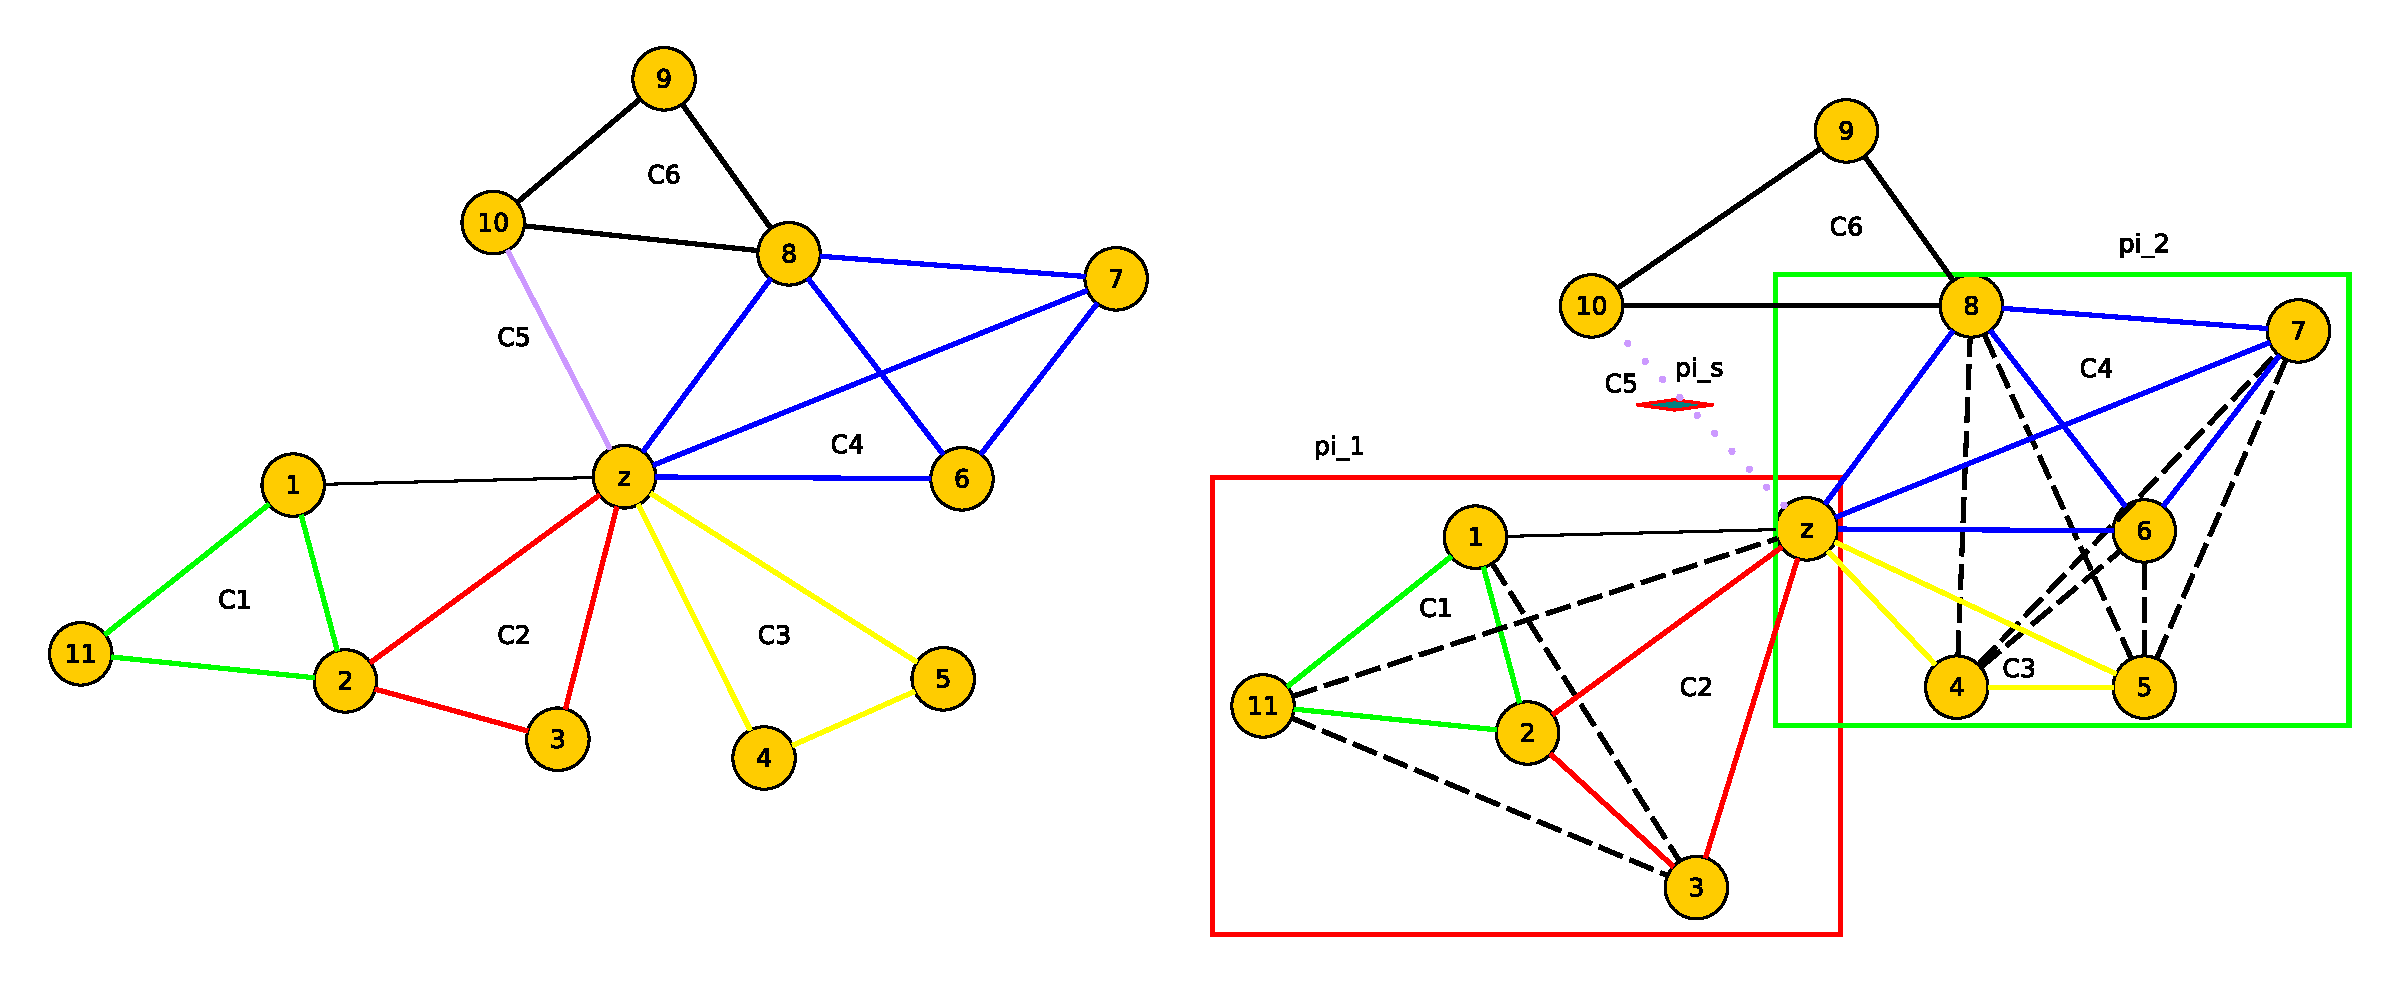
\includegraphics[scale=0.450]{./correctionGraph.eps} \vspace{-0.5em}
\caption{(a) Le sommet $z$ et son voisinage avec les cliques qui le couvrent , (b) un exemple de compression de cliques :  les sommets \`a l'int\'erieur des rectangles rouges et verts forment les nouvelles cliques couvrant $z$.
		$\pi_1 = \{1,2,3,z,11\}$, $\pi_2 = \{z,4,5,6,7,8\}$, $\pi_s = \{10\}$ 
		}
\label{exempleAlgoCorrectionGraphe}
\end{figure}
%% ------ figure correctionGraph
\FloatBarrier

Soient $\pi_1$, $\pi_2$ une bipartition du voisinage du sommet $z_i$  en cliques  et 
$\pi_s$ un ensemble  de sommets dont l'ar\^ete form\'ee par un de ces sommets et le sommet $z_i$ sont  \`a retirer du graphe $G_c$.  
\begin{definition}
Soient 
${\cal CC}^{i}$ la couverture de corr\'elation apr\`es le traitement des $(i-1)^{ieme}$ sommets de ${\cal C}$ et
${\cal CC}^{i}(z_i)$ l'ensemble des cliques contenant le $i^{ieme}$ sommet $z_i$.
\newline
On appelle {\bf compression} du sommet $z_i$ un triplet ($\pi_1$, $\pi_2$, $\pi_s$) d\'efini par : 
\begin{itemize}
	\item $\pi_1$ (resp. $\pi_2$) peut \^etre d'une des formes suivantes :
	\begin{enumerate}
		\item L'union de $z_i$, d'un sous-ensemble $C_1$ (resp. $C_2$) de cliques de ${\cal CC}^{i}(z_i)$ telle que toute paire $(C,C')$ de $C_1$ (resp. $C_2$) est contractable et d'un sous-ensemble $S_1$ (resp. $S_2$) de sommets $v \in S(z_i)$ n'appartenant \`a aucune clique de $C_1$ (resp. $C_2$) tel que
		$$ \forall v \in S_1,~\forall x \in C_1, \not\exists C' \in {\cal CC}^{i}~t.q.~card(C')>2~~et~~\{v,x\} \subset C'$$
		(ce qui fait que \{v,x\} peut \^etre une clique de ${\cal CC}^{i}$).
		\item Une augmentation du sommet $z_i$.
	\end{enumerate}
	\item L'intersection entre $\pi_1$ et $\pi_2$ est r\'eduite $\{z_i\}$ ($\pi_1 \cap \pi_2 = \{z_i\}$),
	\item $\pi_s=\Gamma_{G_c}(z_i)-~((\pi_1 \cap \Gamma_{G_c}(z_i) ) \cup(\pi_2 \cap \Gamma_{G_c}(z_i) ))$ tel que l'ensemble des ar\^etes  $\{[z_i,v]\in E_{c}^{i}:~v\in \pi_s\}$ n'est pas d\'econnectant.
	\item Le triplet $\pi_{1} \cap \Gamma_{G_c}(z_i)$, $\pi_{2} \cap \Gamma_{G_c}(z_i)$, $\pi_{s} \cap \Gamma_{G_c}(z_i)$  est une 3-partition de $\Gamma_{G_c}(z_i)$.
\end{itemize}
\end{definition}
Il existe toujours une telle compression, ne serait-ce que 
$\pi_1 = \{z_i\} \cup C_i \in C(z_i)$, 
$\pi_2 =  \emptyset$,
$\pi_s = \Gamma_{G_c}(z_i) -(\Gamma_{G_c}(z_i) \cup C_i) $  si ${\cal CC}^{i}(z_i)$ n'est pas vide.
Sinon, 
$\pi_1 = \{z_i\} \cup \{ v \in \Gamma_{G_c}(z_i)  \} $, 
$\pi_2 =  \emptyset$,
$\pi_s = \Gamma_{G_c}(z_i) - \{v\} $
est aussi une compression.
Un exemple de compression est aussi donn\'e dans la figure \ref{exempleAlgoCorrectionGraphe}.
Le co\^ut $c(T)$ d'une compression $\pi_{1},\pi_{2},\pi_{s}$ est d\'efini par : 
$$c(T) = | \{\{u,v\} \in \pi_{1}:~[u,v]\not\in E_{c}^{i}\}| + |\{\{u,v\} \in \pi_2:~[u,v]\not\in E_{c}^{i}\}| +~ |\pi_s| $$
%Dans l'exemple de la figure \ref{exempleAlgoCorrectionGraphe}(b), autour d'un sommet $z_i$, l'ensemble $C(z_i)$ contient les cliques $C2$, $C3$,$C4$ et $C5$.
%Les cliques $C5$ et $C4$ ne sont pas contractables, \`a cause de l'existence de $C6$ dans ${\cal C}_i$.
%La clique $C1$ est voisine de $z_i$ et $D_{z_i}(C1) = \{C2\}$.
L'exemple de la compression donn\'ee dans la figure \ref{exempleAlgoCorrectionGraphe}(b) est $\pi_1 = C1 \cup C2$ (une augmentation), $\pi_2 = C3 \cup C4$ (ces deux cliques \'etant contractables), et $\pi_s = \{10\}$.
Les cliques $C1$ et $C2$ sont compress\'ees en ajoutant les ar\^etes $[1,3]$ et $[z_i,11]$. De m\^eme, les cliques $C3$ et $C4$ sont compress\'ees en ajoutant les ar\^etes  $[4,8]$, $[5,8]$, $[7,4]$, $[7,5]$, $[6,4]$ et $[6,5]$. La clique $C5$ est supprim\'ee afin que $z_i$ ne soit pas couvert par trois cliques.
Le co\^ut  de cette compression est $10$, $10$ \'etant le nombre d'ar\^etes en pointill\'ees plus l'ar\^ete supprim\'ee $[10,z_i]$.
\newline

Soit  $c(T)$ le co\^ut minimum d'une compression $T$ de $z_i$.
Le but est de modifier $G_c$ afin que $z_i$ puisse \^etre couvert par une ou deux cliques issues de $\pi_1$ et $\pi_2$.
Pour cela, le co\^ut de cette modification $c(T)$ tient compte des ar\^etes \`a ajouter (li\'ees \`a $\pi_1$ et $\pi_2$) et \`a supprimer (li\'ees \`a $\pi_s$).
\begin{equation}
c(T) = \sum_{ \{u,v\} \subseteq \pi_1: [u,v] \notin E_c^i } \phi^{+}(u,v) + \sum_{ \{u,v\} \subseteq \pi_2: [u,v] \notin E_c^i } \phi^{-}(u,v) + \sum_{ v \in \pi_s } \phi^{-}(u,v)
\end{equation}
Avec $\phi^{+}$ le co\^ut de l'op\'eration {\em ajouter une ar\^ete} et  
$\phi^{-}$ le co\^ut de l'op\'eration {\em ajouter une ar\^ete}.
\newline
Nous \'evaluons les performances des diff\'erents couples de fonctions $\phi^{+}$ et $\phi^{-}$ dans le chapitre \ref{chapitreEvaluation}.
\newline

Ainsi, {\bf appliquer une compression} $T = \pi_1, \pi_2, \pi_s$ consiste \`a ajouter dans $E_c^i$ les ar\^etes d\'efinies par les ensembles de paires $\{\{u,v\} \in \pi_1:~[u,v]\not\in E_{c}^{i}\}$ (qui seront couvertes par la clique $\pi_1$) et $\{\{u,v\} \in \pi_2:~[u,v]\not\in  E_{c}^{i}\}$ (qui seront couvertes par la clique $\pi_2$) et \`a supprimer les ar\^etes $\{[z_i,v] \in  E_{c}^{i}:~v\in \pi_S\}$. 
\newline
D\`es lors, le sommet $z_i$ appartient aux deux cliques $\pi_1$ et $\pi_2$.
On proc\`ede alors aux mises \`a jour suivantes pour obtenir ${\cal CC}^{i+1}$ et $E_M^{i+1}$ :
\begin{itemize}
\item Supprimer toutes les cliques ${\cal CC}^{i}(z_i)$ couvertes par $\pi_1$ dans  ${\cal CC}^{i}$.
\item Supprimer toutes les cliques ${\cal CC}^{i}(z_i)$ couvertes par $\pi_2$ dans  ${\cal CC}^{i}$.
\item Supprimer toutes les cliques de cardinalit\'e $2$ couvertes par $\pi_1$ et $\pi_2$ dans  ${\cal CC}^{i}$.
\item Ajouter $\pi_1$ et $\pi_2$ dans ${\cal CC}^{i}$, supprimer de $E_c^{i+1}$ toutes les ar\^etes  $\{[z_i,v] \in E_c^{i}:~v\in \pi_s\}$.
\item Affecter $Cliq(z)$ \`a $1$ (si $\pi_1$  ou $\pi_2$ est vide) ou $2$ (sinon).
\end{itemize}
Cette proc\'edure a les propri\'et\'es suivantes :
\begin{property}
Consid\'erons l'application d'une compression.\newline
Soit ${\cal CC}^{i+1}$  l'ensemble obtenu \`a partir de ${\cal CC}^{i}$ apr\`es  la mise \`a jour selon cette application.
\begin{itemize}
	\item Tout sommet de $G_c$ couvert par une ou deux cliques dans ${\cal CC}^{i}$ le reste dans ${\cal CC}^{i+1}$.
	\item Toute ar\^ete couverte par une et une seule clique dans ${\cal CC}^{i}$ et qui n'est pas supprim\'ee le reste dans ${\cal CC}^{i+1}$.
	\item Le sommet $z_i$ est couvert par une ou deux cliques dans ${\cal CC}^{i+1}$ (le nombre de sommets ainsi couverts augmente de $1$ par rapport \`a celui dans ${\cal CC}^{i}$).
\end{itemize}
\end{property}

Ainsi, pour chaque sommet $z_i$, on consid\`ere une compression de co\^ut minimum $c_m^i$ et on l'applique.
La propri\'et\'e ci-dessus garantit qu'\`a la fin du processus, on obtient un graphe de corr\'elation $G_c^t = (V_c, E_c^t)$ dont l'ensemble ${\cal CC}^{i}$ modifi\'e est une couverture de corr\'elation.
Consid\'erons la distance de correction $DC(G_c^0, G_c^t ) = | (E_c^0 \cup E_c^t)  - (E_c^0 \cap E_c^t) |$ qui est le nombre de cases modifi\'ees dans la matrice d'adjacence du graphe $G_c$.
La distance-line v\'erifie  
$$DL( G_{c}^{0}, G_{c}^{t}) \le  DC(G_c^0, G_c^t ) $$
Notons que lors d'une \'etape $j > 1$, le sommet $z_j$ et son voisinage se retrouvent \^etre couvert par une ou deux cliques suite au traitement des $j-1$ sommets pr\'ec\'edents, aucune compression ne lui est appliqu\'ee (on consid\`ere la compression identit\'e) et donc 
$c_{m}^{j} = 0$.